\chapter{Koordinaatio}

\begin{figure}[t]
\centering 
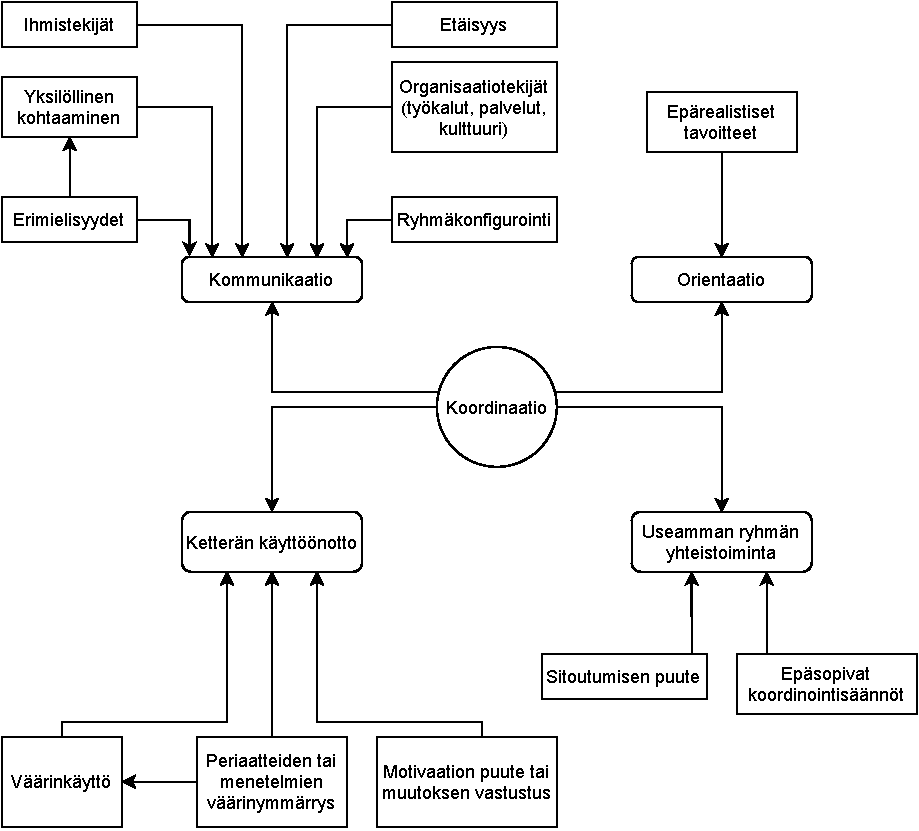
\includegraphics[width=0.9\textwidth]{template/figures/koordinaatiohaasteet.pdf}
\caption{Kaavio koordinaatiohaasteista ja niiden tekijöistä perustuen Alzoubi et al. \cite{ALZOUBI201622}, de Melo et al. \cite{DEOMELO2013412}, Gregory et al. \cite{GREGORY201692}, Moe et al. \cite{MOE2012853} ja Silva et al. \cite{SELLERISILVA201520} tutkimuksiin.\label{fig:koordinaatiohaasteet}}
\end{figure}

Koordinaatiota voidaan tarkastella suurimpana vaikuttavana alueena ketterää ohjelmistokehitystä noudattavassa ryhmässä. Aihetta voidaan ajatella koko toimintaketjun sitovana liimana, sillä valtaosan esitettävistä aihealueista voidaan tulkita kuuluvan koordinaation alle. Tämä tutkielma jaottelee ryhmän koordinaatiohaasteet ketterän käyttöönottoon, kommunikaatioon, useamman ryhmän väliseen koordinaatioon sekä orientaatioon. Koordinaatio aiheena kattaa kaiken, joka voidaan tulkita vaikuttavan kehitysryhmän sisäiseen tai ulkoiseen yhteistoimintaan. Ryhmän sisäiseksi koordinaatioksi tulkitaan tässä kontekstissa ryhmäläisten välinen interaktio, kun taas ulkoiseksi koordinaatioksi tulkitaan esimerkiksi organisaation puolelta tuleva ohjeistaminen (tai ohjaus), mahdollisten muiden saman projektin parissa työskentelevien ryhmien kanssa yhteistyöskentely ja asiakkaan kanssa toimiminen. Esimerkkitapaus ulkoisesta koordinaatiosta on projekti, joka toteutetaan maailmanlaajuisesti hajautetulla ketteränä ohjelmistokehityksenä \cite{ALZOUBI201622}. Esitettävät haasteet voidaan tulkita vaikuttavan voimakkaammin niin laajemmissa ja maailmanlaajuisesti hajautetuissa ketterän kehityksen ryhmissä verrattuna niin sanotusti paikalliseen ryhmään. Maailmanlaajuisesti hajautettu ketterä kehitys tarkoittaa sitä, että prosessi koostuu ryhmistä tai ryhmäläisistä, jotka sijaitsevat maantieteellisesti kaukana toisistaan. Paikallinen ketterä kehitys tarkoittaa tässä kontekstissa vastakohtaa. Koordinaation ollessa varsin laaja käsite, siihen on yhdistettävissä lukuisia mahdollisia haasteita aina yhteistoiminnan käyttöönotosta ylläpitoon. Tulevissa alakappaleissa tutkielma esittelee kuvan \ref{fig:koordinaatiohaasteet} mukaisesti yleisimmät koordinaatiohaasteet, niiden tekijöitä ja vaikutuksia sekä mahdollisia ratkaisumalleja.

\section{Ketterän käyttöönotto}

Ensimmäisenä haasteena ketterän koordinointiin liittyen on ketterän menetelmän käyttöönotto ja siispä ketteriä periaatteita noudattavan ryhmän luonti. Eräänä haasteena käyttöönottoon liittyen on todettu tilanne, jossa perinteisiä malleja, kuten vesiputousta harjoittanut organisaatio haluaa ketteryyttä pohjautuen tietoon, että ketterä tuottaa parempaa kilpailukykyä \cite{MCKNIGHT2014168}. Haasteita tässä tapauksessa voi tuottaa organisaation ymmärrystaso ketteristä periaatteista ja niiden toteutustavoista. Puutteellinen ymmärrys voi olla seuraamusta käyttöönottoon liittyvästä puutteellisesta motivaatiosta, joka juontaa juurensa menetelmätottumuksiin \cite{GREGORY201692}. Syynä voi olla myös muutoksen vastustus tai liian haastelähtöinen näkökulma ketterään kehitykseen, kuten \cite{SELLERISILVA201520} toteavat. Mikäli organisaatiossa ei ymmärretä ketteryyteen liittyviä hyötyjä, siihen liittyviä riskejä tai varsinaisia toteutusmenetelmiä on odotettavissa haastava tie käyttöönoton suhteen.

Tutkimuksessaan Gregory et al. \cite{GREGORY201692} toteavat haasteita liittyen ketterän toteuttamiseen ja käyttöönottoon perinteisen ympäristön ja organisaation kontekstissa. Eräänä rajoittavana tekijänä käyttöönottoon liittyen todettiin ketterän väärinkäyttö, joka johtuu väärinymmärryksestä. Tutkimuksessa ilmeni tilanne väärinkäytöstä, missä organisaation johto on teettänyt niin sanotun ketterän ryhmän työskentelemään massiivisen määrän ylitöitä perustellen sen olevan osana ketterää menetelmää. Skenaariossa on nähtävissä kehittäjien loppuunpalaminen sekä organisaation paluu perinteisten menetelmien käyttöön, kun uusi menetelmä ei olekaan tuottanut odotettua tulosta. Toisena väärinkäyttöön liittyvänä skenaariona ilmeni tilanne, jossa jonkin ketterän menetelmän käyttöönoton jälkeen organisaation johto on alkanut mikromanageroimaan kehitysryhmää ainakin siihen saakka, kunnes nähtävää tulosta on alkanut muodostumaan. Jatkuvan mikromanageroinnin seurauksena on nähtävissä varsinaisen ketteryyden ja sen sisältävän luovuuden väheneminen. Toisaalta ohjaukseen liittyen Silva et al. \cite{SELLERISILVA201520} toteavat olevan oleellista tukea ja ohjata ketterän käyttöönottoa aikaisissa vaiheissa.

Käyttöönottohaasteiden minimoimiseksi on todettu olevan suositeltavaa hakea konsultointia ammattilaisilta ja yrityksiltä, joilla on tunnustettua erityisosaamista ketterään kehitykseen liittyen \cite{SELLERISILVA201520}. Siispä ratkaisuna haasteelle voidaan ajatella olevan tehokasta perehtyä kattavasti ketteriin periaatteisiin ja käyttöönotettavaan menetelmään. Silva et al. \cite{SELLERISILVA201520} muistuttavat lisäksi, että ketterien periaatteiden mukaisesti ketterän kehitysryhmän tulisi pyrkiä itse esittämään ratkaisumalleja ongelmatilanteisiin.

\section{Kommunikaatio}

Kommunikaation voidaan ajatella olevan ketterän ryhmän koordinaation mahdollistava työkalu. Ilman kommunikaatiota ei olisi yhteistoimintaa, ainakaan tehokkaanlaatuista. Alzoubi et al. \cite{ALZOUBI201622} korostavat kommunikaation tehokasta käyttöönottoa alusta alkaen muiden haasteiden välttämiseksi. Haasteiden minimoimiseksi olisi olennaista, että ketterä ryhmä kommunikoi ryhmäläistensä kesken ja ryhmän ulkopuolella olevien yhteistyötahojen kanssa. Kommunikaation merkitys korostuu maantieteellisesti hajautettujen ryhmien osalta, sillä kyseiset kehittäjät eivät lähtökohtaisesti pääse samaan työskentelytilaan muiden kanssa. Ketterien periaatteiden korostaessa asiakasyhteistyötä on myös ratkaisevaa, että ryhmä kommunikoi asiakkaan kanssa riittävän selkeästi ja usein.

Tutkimuksessaan Alzoubi et al. \cite{ALZOUBI201622} keskittyvät ketterään liittyvän kommunikaatioon ja tuovat esille siihen liittyviä haasteita ja ratkaisumalleja. Tutkimus itsessään keskittyy maailmanlaajuisesti hajautetun ketterän ohjelmistokehityksen kommunikatiivisiin seikkoihin, mutta tuloksia voidaan soveltaa paikallisesti toteutettavaan variaatioon oletuksella, että paikallisvariaatiossa haasteet ovat lievempiä. Tutkimuksessa puutteellisen kommunikoinnin todettiin johtavan kaikkiin muihin haasteisiin ja niiden käsittelyn vaativan 2,5 kertaa enemmän resursseja kuin paikallisessa variaatiossa. Alzoubi et al. toteavat ketterän kehityksen nojaavan epävirallisiin kommunikointikeinoihin ryhmäläisten välillä, sillä kommunikoinnin on todettu olevan huomattavasti tehokkaampaa epävirallisten menetelmien pohjalta. Epäviralliset kommunikointimenetelmät voidaan jakaa henkilökohtaiseen, vuorovaikutteiseen ja vertaisorientoituneeseen tapaan. Epävirallisen kommunikoinnin on todettu nojaavan voimakkaasti vuorovaikutukseen, joka tapahtuu kasvotusten niin ryhmäläisten kuin ryhmän ja asiakkaan välillä. Tästä johtuen ryhmäläisten välinen sijainti korostuu voimakkaasti vaikuttavana tekijänä.

Alzoubi et al. tutkimuksessa \cite{ALZOUBI201622} todettiin, että lähteinä kommunikointihaasteille ovat muun muassa etäisyys, organisaatiotekijät, ihmistekijät ja ryhmäkonfigurointi. Etäisyyden todettiin olevan yleisin haasteiden lähde. Sen todettiin hankaloittavan koordinaatiota esimerkiksi viiveinä kommunikoinnissa, pidempinä kokouksina, hankaluutena löytää yhteisiä työaikoja ja luottamuksen puutteena. Silva et al. tutkimuksessa \cite{SELLERISILVA201520} todettiin rajoittavana tekijänä ryhmän sisäiset erimielisyydet, joiden voidaan olettaa hankaloittavan kommunikointia. Ryhmäkonfigurointiin liittyen sekä \cite{SELLERISILVA201520} että \cite{ALZOUBI201622} toteavat kommunikoinnin hankaloituvan sen mukaan, mitä suurempi ryhmä on kyseessä. Sama pätee myös tapaukseen, jossa projektin parissa työskentelee useampi ryhmä. Lisäksi Alzoubi et al. \cite{ALZOUBI201622} toteavat, että satunnaisissa tapauksissa jotkin ryhmäläiset eivät halua kommunikoida ja omaavat huonomman ymmärryksen koordinaatiosta. Kommunikoinnin haluttomuuteen liittyy myös Moe et al. \cite{MOE2012853} tutkimus, jossa todetaan haasteena ryhmäläisten keskinäinen kohtaaminen. Ryhmäläiset eivät välttämättä halua väitellä keskenään, vaan mieluummin mukautuvat tilanteeseen. Seurauksena haasteista ryhmäkonfiguraatiossa on muun muassa aikaisen vaiheen kommunikointiongelmat, ryhmäläisten haluttomuus ryhmäkommunikointiin, vähentynyt ymmärrys ryhmätyöskentelystä sekä hitaus kommunikoinnissa \cite{ALZOUBI201622}. Lisäksi keskinäisen kohtaamattomuuden seurauksena on ryhmän tehoton päätöksenteko \cite{MOE2012853}. Organisaatiotekijöiksi listattiin organisaation työkalut ja palveluiden kyky tukea kommunikointia \cite{ALZOUBI201622}. Työkaluihin ja palveluihin lukeutuvat muun muassa puhelin, pikaviestipalvelut sekä sähköposti. Merkittäväksi tekijäksi on listattu myös organisaation kulttuuri, joka koostuu asenteista, arvoista ja käytänteistä. Seurauksena organisaatiotekijöistä ovat muun muassa tehottomampi ryhmä, huonolaatuisempi ohjelmisto, suurempi määrä työkaluja sekä puutteellinen luotto.

Ratkaisumalleiksi Alzoubi et al. \cite{ALZOUBI201622} listaavat seuraavanlaista. Ryhmäkonfiguraatiosta lähtöisin oleviin haasteisiin strategiaksi ehdotetaan ensinnäkin paikallisten tapaamisten järjestämistä. Paikallisten tapaamisten on todettu tuottavan epävirallisempaa kommunikointia, joka tehostaa ryhmän tuottavuutta \cite{DEOMELO2013412}. Toisaalta \cite{ALZOUBI201622} listaavat samalla osaksi strategiaa tehokkaan virallisen kommunikoinnin lisäämisen. Muita osia strategiasta ovat muun muassa projektin säännöllinen esittely osapuolille, säännöllisten tapaamisten järjestäminen, paikallisten ryhmien muodostus sekä selkeiden roolien ja vastuiden jako. Toisaalta \cite{CLAPS201521} toteavat roolien jakoon liittyen erittäin oleelliseksi oikeanlaisen ohjauksen mahdollisen johdon puolelta, ettei prosessi ole vahingollinen ryhmille. Claps et al. \cite{CLAPS201521} korostavat roolijaon olevan itsessään haastava tehtävä. Organisaatiotekijöistä lähtöisin oleviin haasteisiin Alzoubi et al. \cite{ALZOUBI201622} ehdottavat strategiaksi korostaa työskentelykulttuuria, joka suosii jatkuvaa kommunikointia, luottoa sidosryhmien välillä sekä nopeaa asiakaspalautetta. 

\section{Useamman ryhmän yhteistoiminta}

Tutkimuksessaan de Melo et al. \cite{DEOMELO2013412} toteavat ketterän ryhmän tuottavuuden koostuvan ryhmän sisäisistä ja ulkoisista tekijöistä. Ryhmän ulkoiset tekijät rajautuvat useamman ryhmän väliseen koordinaatioon. On todettu, että useista kehitysryhmistä koostuvien projektien ryhmien välinen koordinaatio on yksi hankalimmista kehitettävistä asioista ohjelmistotuotantoon liittyen. Ryhmien välisen koordinoinnin haasteita aiheuttavat sitoutumisen puute sekä epäsopivat koordinointisäännöt ryhmien välillä. Haasteiden on todettu aiheuttavan suuntausvirheitä ja ketteryyden rikkoutumisen. Esimerkkinä suuntausvirheestä toimii tilanne, jossa ryhmän työskentely riippuu toisen ryhmän tuloksista, eivätkä ryhmät työskentele samassa tahdissa. Tällöin syntyy tilanteita, joissa toisesta ryhmästä riippuva ryhmä joutuu odottamaan tai hidastamaan tahtiaan merkittävästi. Toisesta ryhmästä riippuvuuden on todettu olevan yleinen ilmiö laajemmissa ohjelmistoprojekteissa.

Laajojen, useista kehittäjäryhmistä koostuvien projektien osalta on todettu olevan haastavaa toteuttaa laaja-alaista ketterää kehitystä \cite{DEOMELO2013412}. Kaikki ryhmät eivät välttämättä noudata ketteriä periaatteita tai käytä mitään ketterää menetelmää. De Melo et al. \cite{DEOMELO2013412} toteavat, että ketterän ryhmän on äärimmäisen hankalaa tai jopa mahdotonta vaikuttaa muiden ryhmien työskentelymenetelmiin. Täten tilanne, jossa osa ryhmistä käyttää eri ketteriä menetelmiä, osa vaikkapa vesiputousmallia, on mahdollinen. Projektin useat eri kehitysmenetelmät voivat aiheuttaa massiivisia koordinointiongelmia. De Melo et al. mainitsevat ratkaisuna useamman ryhmän yhteistoimintaan ketterän ryhmän kyvyn mukautua erilaisiin tilanteisiin. Mukautumisen kautta voisi olla mahdollista löytää paremmin yhteisiä työskentelytapoja eri menetelmiä käyttävien ryhmien kanssa erityisesti tilanteessa, jossa kumpikin (tai useampi) osapuoli noudattaa jotain ketterää menetelmää. Claps et al. \cite{CLAPS201521} mainitsevat, ettei ryhmien välinen koordinaatio olisi toiminut uuden ketterän menetelmän käyttöönoton kontekstissa ilman johdon käyttöönottamaa strategiaa. Organisaation johdon selkeän strategian myötä kullekin ryhmälle saatiin yhteinen tavoite, jonka myötä ryhmät työskentelivät samaa päämäärää kohti.

\section{Orientaatio}

Tutkimuksessaan Moe et al. \cite{MOE2012853} toteavat yhtenä koordinaatiohaasteena olevan ryhmäorientaation puute. Ryhmäorientaatio tarkoittaa ryhmän yhteistä suuntaa ja sen toteuttaminen tarkoittaa sitä, että kukin ryhmässä työskentelee yhteistä päämäärää kohti. Tutkimuksen mukaan joissain tilanteissa ketterän ryhmän orientaatio voi olla alhainen epärealististen tavoitteiden takia. Alhaisen ryhmäorientaation myötä on todettu tapauksia, joissa yksittäiset ryhmäläiset tekevät omia päätöksiä projektin suhteen sen sijaan, että päätöksistä sovittaisiin yhdessä. Samaten ongelmien raportoinnin on todettu jäävän vähemmälle johtuen siitä, että alhaisen orientaation myötä projektiin liittyviä ongelmia pidetään enemmän henkilökohtaisina kuin ryhmän ongelmina. Kaiken kaikkiaan alhainen ryhmäorientaatio vähentää ryhmän kommunikointia merkittävästi ja sen voidaan tulkita lisäävän riskiä ryhmäläisten siiloutumiselle. Siiloutumisella tarkoitetaan sitä, että jokin osa ryhmästä alkaa työskentelemään suljetusti keskenään ilman muuta osaa ryhmästä.
